\documentclass{article}
\usepackage[utf8]{inputenc}
\usepackage{graphicx}
\usepackage{listings}
\usepackage{float}
\usepackage{indentfirst}
\usepackage{xcolor}
\usepackage{fmtcount}
\usepackage{geometry}
\geometry{margin=1in}

\title{EEL 4712C - Digital Design: Lab Report 3}
\author{Cole Rottenberg \\ 11062528}
\date{\today}

\lstset{
  language=VHDL,
  numbers=left,
  stepnumber=1,
  tabsize=2,
  numbersep=5pt,
  backgroundcolor=\color{white},
  showspaces=false,
  showtabs=true,
  frame=single,
  rulecolor=\color{black},
  captionpos=b,
  breaklines=true,
  breakatwhitespace=true,
  title=\lstname,
}

\begin{document}

\maketitle

\section*{Prelab Report}
\begin{enumerate}
  \item Part 1: One Process FSM
  \item Part 2: Two Process FSM
  \item Part 3: Demo
  \begin{enumerate}
    \item Test on hardware.
    \item Assign inputs and outputs to the switches and LEDs.
    \item Display to TA Fib(11) = 89.
  \end{enumerate}
\end{enumerate}
\subsection*{Prelab Questions}
% Put all the answers to the prelab questions. These may be scanned using your phone or scanner. Not all prelabs have prelab questions
\textbf{Highlighting the key differences between a one process and two process FSM.}
The major difference between a one process and two process FSM is the flow of states and the logic that controls when a state change occurs. In a one process FSM, our sensitivity list contains a \textbf{clk and rst} signal. This means that the state machine will only change states when the clock signal changes. In a two process FSM, our sensitivity list contains the \textbf{state and input(s)} signals. This means that the state machine will change states when the state or input signals change. However, the state change in a two process FSM is iterated by a clock signal. This means that the state machine will only change states when the clock signal changes. This adds a layer of abstraction to the state machine, allowing for more complex state machines to be designed.

\subsection*{Prelab Design and Implementation}
% Go into detail about how you designed any design parts of the prelab. Then, go into detail about how you implemented any implementation parts of the prelab
The design process started with analyzing the given pseudo code and diagram of components of the Fibonacci Sequence from Lab 2. Then I was able to come up with a basic implementation of a state machine picture in figure \ref{fig:state-diagram}. The state machine controls the enable of need register \textbf{i,x,y, and n} and the select lines of multiplexer for \textbf{i,x,y, and n}. The both state machines work by first checking for input signals such as \textbf{go and rst} before moving to an initial state. The initial loads the \textbf{n} register with the input value while other register loads base values for loops and arithmetic. The FSM then checks the \textbf{n} register for a zero value, if it is zero, the FSM moves to the final state and outputs a preset zero value. Otherwise, the FSM moves to the next state and begins the iterative process of calculating the Fibonacci Sequence. The a state checks if we have iterated up to the input value, if so we move to the done state. If we have not, we move to the compute stage which loads the \textbf{y} register into the \textbf{x} register. The FSM then moves to ADD state which loads the summation of \textbf{x} and \textbf{y} registers into the \textbf{y} register. We do so in two seperate states as the addition of the two registers requires a clock cycle. While moving the \textbf{y} register to the \textbf{x} register, we also iterate the \textbf{i} register as to count the number of iterations. We then loop back to the original CHECK state and continue the process until we reach the input value. As mentioned before, if we reach the input value, we move to the done state and output the \textbf{done} signal. Before moving from the done state, we must also check of the original \textbf{go} signal has reached zero. If it has, we move to the restart state which also outputs the \textbf{done} signal. If the \textbf{go} signal is not zero, we stay in the done state until it is zero. From the restart state, we are able to move back to the initial state if we receive a \textbf{go} signal. This is the basic design of the state machine. The implementation of the state machine is done in VHDL and is shown in the appendix. The one process FSM code is shown in listing \ref{lst:one-process-fsm-vhdl-code} and the two process FSM code is shown in listing \ref{lst:two-process-fsm-vhdl-code}.

\subsection*{Reflection} % Talk about what you learned during the prelab. Bring up anything that was a stumped you for a while. Bring up any accomplishments you were proud of.

\subsection*{Prelab Homework}
% Show all work for the Prelab Homework here
% Show all the work for every step in the Prelab Homework section. Label each part clearly and caption all figures. All simulations must be annotated. Annotation means pointing out particularly important parts of a simulation. This can be done with arrows or textboxes. Simple simulations will not have a lot to talk about, but later simulations will be a lot more complex. Any code written in the prelab should be commented a fair amount.

\section*{Postlab Report}

\subsection*{Problem Statement}
% Provide a short informal description of the lab’s goals (From the lab assignment)
% If required, specify the system to design.
% - Define the inputs.
% - Define the outputs.
% - Define the function of your system. 
% This section should be 1-2 paragraphs long.
The goal of the lab was to implement a working FSM to control the datapath implemented in lab 2. The control focused around enabling certain registers and select lines. The inputs used by the FSM include: clk, rst, go, n\_eq\_0, and i\_le\_n. The outputs of the FSM include: done, n\_en, result\_en, result\_sel, x\_en, x\_sel, y\_en, y\_sel, i\_en, and i\_sel. The function of the system is to control the datapath to calculate the Fibonacci Sequence. The FSM controls the enable and select lines of the registers and multiplexers in the datapath. The FSM also outputs the done signal when the computation is complete.

\subsection*{Design}
% Describe the design decisions you made.
% - What components did you use?
% - What signals did you use to connect the components?
% - What algorithms did you use?
% Code Segment or block diagrams may be included here.
% Explain your design choices(pros/cons).
% Any designs made in prelab should be included here but more briefly.
% This section should be 1-2 paragraphs long.

The design of the FSM was based on the state diagram shown in figure \ref{fig:state-diagram}. The FSM was implemented in VHDL and was designed to control the datapath of the Fibonacci Sequence. The FSM was designed to control the enable and select lines of the registers and multiplexers in the datapath. The FSM was also designed to output the done signal when the computation is complete. The FSM was implemented in both a one process and two process design. The one process FSM was implemented to control the datapath as expected. 

\subsection*{Implementation}
% Describe the implementation process.
% Code segments or block diagrams may be included here.
% What time did you need to complete your design?
% This section should be 1-2 paragraphs long.

THe implementation took a much longer time than expected. For both the one process and two process FSMs, the implementation used similar states and internal signals however, the overall expectation of state and signal changes was different. As seen in the code, the one process FSM used a clock and reset signal to control the state changes. The two process FSM used the state and input signals to control the state changes, however the state changes were iterated by a clock signal. The implementation of the FSM took much longer than expected. 

\subsection*{Testing}
% Describe how you tested your design.
% Did everything work as expected?
% - Did inputs match the expected outputs?
% - Special cases?
% Include if possible, timing diagram of photo/video of the system.
The testing of the design was done by first simulating the FSM in ModelSim. The simulation was done by creating a testbench that would simulate the FSM with a set of inputs. The inputs were chosen to test the FSM in a scenario entering a loop and then recieving the \textbf{i\_le\_n} signal. The simulation was successful and the FSM was able to iterate through the states as expected. After recieving the \textbf{i\_le\_n}, the FSM reached the done state and outputted the \textbf{done} signal. We also can observe the individual states of computation by analyzing the enable and select signals of the registers and multiplexers. The testbench code was used for both the one process and two process FSMs. The testbench code is shown in listing \ref{lst:testbench-vhdl-code}. 

\subsection*{Conclusions}
% Summarize in one paragraph, the work you did, the success and problems you encountered, and how to improve next in the future.
% This section should only be 1 paragraph long.

The direction and control of the FSM was eventually successful, however the implementation and testing of the FSM took an extensive amount of time. The overall testing and work to develop the FSM took much longer than expected. We were able to produce a proper fibonacci output after hours and hours of testing and implementation. Both the one process and two process FSMs were implemented and tested. The one process FSM was able to control the datapath as expected. The two process FSM was also able to control the datapath as expected.

\section*{Appendix}
% Include all postlab code, screenshots, and simulations here. ALL SIMULATIONS MUST BE ANNOTATED. This means pointing out particularly important parts of a simulation. This can be done with arrows or textboxes. All figures must be captioned. Code should be commented a fair amount.

% State Diagram
\begin{figure}[H]
  \centering
  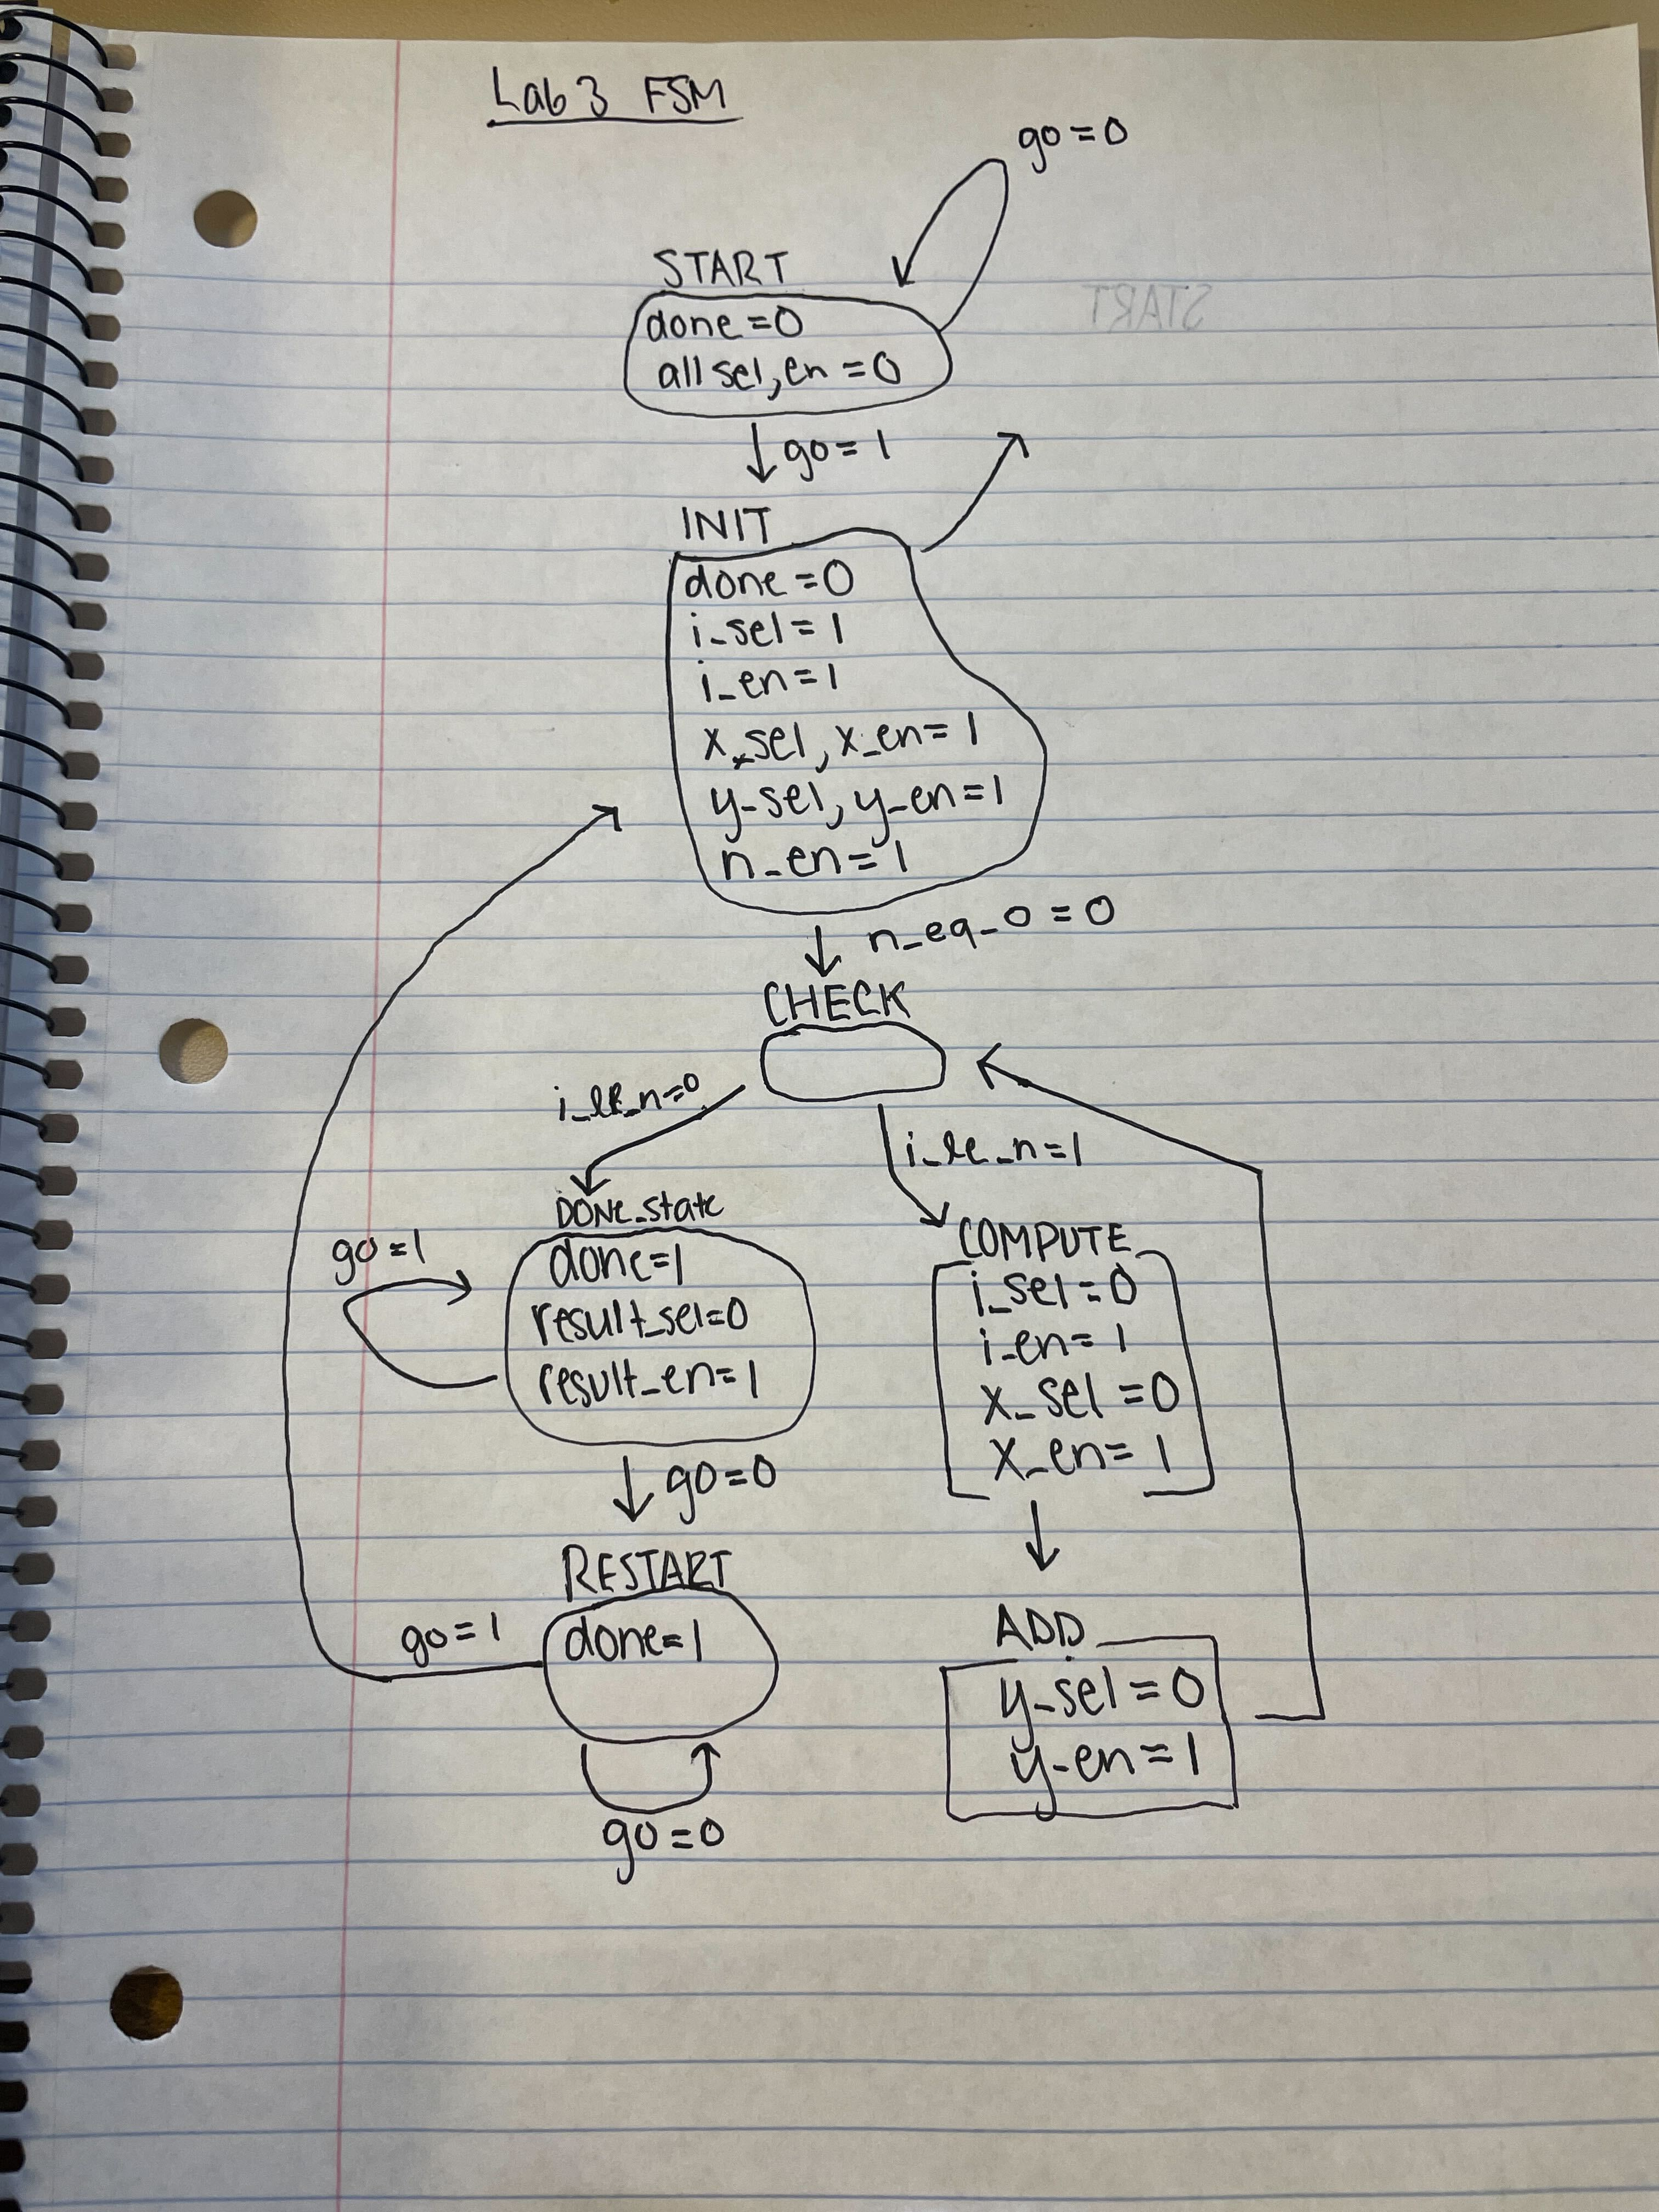
\includegraphics[width=0.5\textwidth]{state_diagram.jpg}
  \caption{State Diagram}
  \label{fig:state-diagram}
\end{figure}

% One Process FSM VHDL Code
\begin{lstlisting}[caption=One Process FSM VHDL Code, label=lst:one-process-fsm-vhdl-code]
library ieee;
use ieee.std_logic_1164.all;
use ieee.numeric_std.all;
-- FSM:
-- Building a FSM for the fibonacci datapath
entity fsm is
    port(
        -- Inputs
        clk:        in std_logic;
        rst:        in std_logic;
        go:         in std_logic;
        n_eq_0:     in std_logic;
        i_le_n:     in std_logic;

        -- Outputs
        done:       out std_logic;
        
        -- Control signals
        n_en:       out std_logic;
        result_en:  out std_logic;
        result_sel: out std_logic;
        x_en:       out std_logic;
        x_sel:      out std_logic;
        y_en:       out std_logic;
        y_sel:      out std_logic;
        i_en:       out std_logic;
        i_sel:      out std_logic
    );
end entity fsm;

architecture behavioral of fsm is
    -- Define the states
    type state_t is (START, INIT, COMPUTE, CHECK_LE, DONE_STATE, RESTART);
    signal state, next_state:       state_t := START;

begin
    -- No Clock Style
    -- Logic for state transitions
    process(clk, rst)
    begin
        if (rst = '1') then
            done <= '0';
            state <= START;
        -- Default values
        -- State transitions
        elsif (rising_edge(clk)) then
            done <= '0';
            i_sel <= '0';
            i_en <= '0';
            x_sel <= '0';
            x_en <= '0';
            y_sel <= '0';
            y_en <= '0';
            n_en <= '0';
            result_en <= '0';
            result_sel <= '0';
            
            case state is
                when START =>
                    -- All to 0
                    done <= '0';
                    i_sel <= '0';
                    i_en <= '0';

                    x_sel <= '0';
                    x_en <= '0';

                    y_sel <= '0';
                    y_en <= '0';

                    n_en <= '0';

                    result_en <= '0';
                    result_sel <= '0';

                    if go = '1' then
                        state <= INIT;
						n_en <= '1';
                    else
                        state <= START;
                    end if;
                -- Implement default defined values for every state

                when INIT =>
                    if (n_eq_0 = '0') then
                        result_sel <= '0'; -- Select the result
                        i_sel <= '1'; -- i become 2... beginning of loop
                        i_en <= '1';

                        x_sel <= '1'; -- X become 0... starting value
                        x_en <= '1';

                        y_sel <= '1'; -- Y become 1... starting value
                        y_en <= '1';
                        state <= CHECK_LE;
                    else
                        result_sel <= '1'; -- Select default 0 result if n = 0
						result_en <= '1'; -- Enable for DONE_STATE
                        state <= DONE_STATE;
                    end if;

                when CHECK_LE =>
                    -- Check if i <= n
                    if (i_le_n = '1') then
                        state <= COMPUTE;
						i_en <= '1';
                    else
                        x_en <= '0';
                        y_en <= '0';
                        i_en <= '0';
                        state <= DONE_STATE;
						result_sel <= '0';
						result_en <= '1';
                    end if;
                
                when COMPUTE =>
                    i_sel <= '0';
                    i_en <= '0'; -- Redundant
                    x_sel <= '0';
                    x_en <= '1'; -- Redundant
                    y_sel <= '0';
                    y_en <= '1'; -- Redundant

                    state <= CHECK_LE;

                when DONE_STATE =>
                    -- Need to prevent bad state loops because of race conditions
                    done <= '1';
                    if go = '1' then
                        state <= DONE_STATE;
                    else
                        state <= RESTART;
                    end if;
                when RESTART =>
 
                    done <= '1';
                    -- Now we can restart the process if go is high
                    if go = '1' then
                        state <= INIT;
						done <= '0';
						n_en <= '1';
                    else
                        state <= RESTART;
                    end if;
                when others => null;
            end case;
        end if;
    end process;
end architecture behavioral;
\end{lstlisting}

% Two Process FSM VHDL Code
\begin{lstlisting}[caption=Two Process FSM VHDL Code, label=lst:two-process-fsm-vhdl-code]
library ieee;
use ieee.std_logic_1164.all;
use ieee.numeric_std.all;

-- FSM:
-- Building a FSM for the fibonacci datapath

entity fsm is
    port(
        -- Inputs
        clk:        in std_logic;
        rst:        in std_logic;
        go:         in std_logic;
        n_eq_0:     in std_logic;
        i_le_n:     in std_logic;

        -- Outputs
        done:       out std_logic;
        
        -- Control signals
        n_en:       out std_logic;
        result_en:  out std_logic;
        result_sel: out std_logic;
        x_en:       out std_logic;
        x_sel:      out std_logic;
        y_en:       out std_logic;
        y_sel:      out std_logic;
        i_en:       out std_logic;
        i_sel:      out std_logic
    );

end entity fsm;

architecture behavioral of fsm is
    -- Define the states
    type state_type is (START, INIT, BUFF, COMPUTE, ADD, CHECK_LE, DONE_STATE, RESTART);
    signal state, next_state:       state_type := START;

begin
    -- Logic for clock and reset 
    process(clk, rst)
    begin
        if rst = '1' then
            state <= START; -- Reset state
        elsif rising_edge(clk) then
            state <= next_state; -- Update state
        end if;

    end process;

    -- Logic for state transitions
    process(state, go)
    begin
        -- Default values to prevent latches
        -- State transitions
        case state is

            when START =>
                -- All to 0
                i_en <= '0';
                x_en <= '0';
                y_en <= '0';
                n_en <= '0';
                done <= '0';

                if go = '1' then
                    next_state <= INIT;
                else
                    next_state <= START;
                end if;
               -- Implement default defined values for every state

            when INIT =>
                -- Unable Done
                done <= '0';
                i_sel <= '1';
                i_en <= '1';
                x_sel <= '1';
                x_en <= '1';
                y_sel <= '1';
                y_en <= '1';
                n_en <= '1';
                result_en <= '0';
                next_state <= CHECK_LE;
            
            when BUFF =>
                -- Buffer state to allow n to loaded and compared
                n_en <= '1';
                next_state <= CHECK_LE;

            when CHECK_LE =>
                -- Check if i <= n
                if (i_le_n = '1') then
                    next_state <= COMPUTE;
                else
                    next_state <= DONE_STATE;
                end if;
            
            when COMPUTE =>
                i_sel <= '0';
                i_en <= '1'; -- Redundant
                x_sel <= '0';
                x_en <= '1'; -- Redundant

                next_state <= ADD;

            when ADD =>
                -- Allows Clock Cycle so the addition of x and y can be done before y is loaded
                y_sel <= '0';
                y_en <= '1'; -- Redundant

                next_state <= BUFF;
            when DONE_STATE =>
                result_sel <= '0'; -- DBG 
                result_en <= '1'; -- Only enable the result... the init state handles which result to select
                -- Need to prevent bad state loops because of race conditions
                done <= '1';
                if go = '1' then
                    next_state <= DONE_STATE;
                else
                    next_state <= RESTART;
                end if;
            when RESTART =>
                result_sel <= '0'; -- DBG 
                result_en <= '0'; -- Only enable the result... the init state handles which result to select
                i_en <= '0';
                x_en <= '0';
                y_en <= '0';
                n_en <= '0';
                done <= '0';
                -- Now we can restart the process if go is high
                if go = '1' then
                    next_state <= INIT;
                else
                    next_state <= RESTART;
                end if;
            when others => null;
        end case;
    end process;
end architecture behavioral;
\end{lstlisting}

% Testbench VHDL Code
\begin{lstlisting}[caption=Testbench VHDL Code, label=lst:testbench-vhdl-code]
  library ieee;
use ieee.std_logic_1164.all;
use ieee.std_logic_arith.all;
use ieee.numeric_std.all;

-- Testbench for the our top_level Fibonacci state machine

entity fsm_tb is
end fsm_tb;

architecture tb of fsm_tb is
  -- Inputs
  signal clk :          std_logic := '0';
  signal rst :          std_logic := '0';
  signal go :           std_logic := '0';
  signal n_eq_0 :       std_logic := '0';
  signal i_le_n :       std_logic := '0';

  -- Outputs
  signal done:          std_logic := '0';

  -- Signals for controlling Datapath
  signal n_en:          std_logic := '0';
  signal result_en:     std_logic := '0';
  signal result_sel:    std_logic := '0';
  signal x_en:          std_logic := '0';
  signal x_sel:         std_logic := '0';
  signal y_en:          std_logic := '0';
  signal y_sel:         std_logic := '0';
  signal i_en:          std_logic := '0';
  signal i_sel:         std_logic := '0';

  -- Datapath inputs

  -- Clock
  constant clk_period : time := 5 ns;

begin
  -- Instantiate the FSM
  UUT : entity work.fsm(behavioral) 
    port map (
      clk => clk,
      rst => rst,
      go => go,
      n_eq_0 => n_eq_0,
      i_le_n => i_le_n,
      done => done,

      n_en => n_en,
      result_en => result_en,
      result_sel => result_sel,
      x_en => x_en,
      x_sel => x_sel,
      y_en => y_en,
      y_sel => y_sel,
      i_en => i_en,
      i_sel => i_sel
    );

  -- Clock process definitions
  clk <= not clk after clk_period;
  
  -- Stimulus process

  process
  begin
    -- Reset
    rst <= '1';
    wait until rising_edge(clk);
    rst <= '0';
    -- Start the FSM
    wait for 10 ns;
    go <= '1';
    i_le_n <= '1';
    wait for 10 ns;

    wait for 100 ns;
    i_le_n <= '0';

    wait for 20 ns;
    go <= '0';
    -- Wait for the FSM to finish
    wait until done = '1'; 

    -- End the simulation
    wait;
  end process;
end tb;library ieee;
use ieee.std_logic_1164.all;
use ieee.std_logic_arith.all;
use ieee.numeric_std.all;

-- Testbench for the our top_level Fibonacci state machine

entity fsm_tb is
end fsm_tb;

architecture tb of fsm_tb is
  -- Inputs
  signal clk :          std_logic := '0';
  signal rst :          std_logic := '0';
  signal go :           std_logic := '0';
  signal n_eq_0 :       std_logic := '0';
  signal i_le_n :       std_logic := '0';

  -- Outputs
  signal done:          std_logic := '0';

  -- Signals for controlling Datapath
  signal n_en:          std_logic := '0';
  signal result_en:     std_logic := '0';
  signal result_sel:    std_logic := '0';
  signal x_en:          std_logic := '0';
  signal x_sel:         std_logic := '0';
  signal y_en:          std_logic := '0';
  signal y_sel:         std_logic := '0';
  signal i_en:          std_logic := '0';
  signal i_sel:         std_logic := '0';

  -- Datapath inputs

  -- Clock
  constant clk_period : time := 5 ns;

begin
  -- Instantiate the FSM
  UUT : entity work.fsm(behavioral) 
    port map (
      clk => clk,
      rst => rst,
      go => go,
      n_eq_0 => n_eq_0,
      i_le_n => i_le_n,
      done => done,

      n_en => n_en,
      result_en => result_en,
      result_sel => result_sel,
      x_en => x_en,
      x_sel => x_sel,
      y_en => y_en,
      y_sel => y_sel,
      i_en => i_en,
      i_sel => i_sel
    );

  -- Clock process definitions
  clk <= not clk after clk_period;
  
  -- Stimulus process

  process
  begin
    -- Reset
    rst <= '1';
    wait until rising_edge(clk);
    rst <= '0';
    -- Start the FSM
    wait for 10 ns;
    go <= '1';
    i_le_n <= '1';
    wait for 10 ns;

    wait for 100 ns;
    i_le_n <= '0';

    wait for 20 ns;
    go <= '0';
    -- Wait for the FSM to finish
    wait until done = '1'; 

    -- End the simulation
    wait;
  end process;
end tb;
\end{lstlisting}

\end{document}
